\documentclass[11pt]{article}

% --- packages ---
\usepackage[margin=1in]{geometry}
\usepackage{amsmath,amssymb,amsfonts}
\usepackage{booktabs}
\usepackage{graphicx}
\usepackage{hyperref}
\usepackage{xcolor}
\usepackage{multirow}
\usepackage{float}
\usepackage[numbers]{natbib}
\usepackage{microtype}
\usepackage{bookmark}
\usepackage{tikz}
\usetikzlibrary{arrows.meta, positioning, fit, backgrounds}

\hypersetup{
  colorlinks=true,
  linkcolor=blue!60!black,
  citecolor=blue!60!black,
  urlcolor=blue!60!black
}

% --- metadata ---
\title{%
  Pure Number Architecture:\\
  Structured Edge Weights Amplify FCC Lattice Topology\\
  Advantages Through Bottleneck Resilience%
}

\author{%
  Timothy Paul Bielec\thanks{Corresponding author: \texttt{timothy@promptcrafted.com}}\\
  Promptcrafted LLC\\
  Los Angeles, CA
}

\date{March 2026}

\begin{document}

\maketitle

% ===================================================================
\begin{abstract}
A companion paper~\cite{bielec2026shape} established that the
face-centered cubic (FCC) lattice provides a $2.3\times$ algebraic
connectivity advantage over the simple cubic (SC) lattice under
uniform edge weights. This paper asks whether structured edge
weights amplify or attenuate that advantage. Seven experiments
across two registers---lattice-scale tessellation and single-cell
characterization---answer definitively: structured weights amplify.
Direction-based weighting, motivated by the rhombic dodecahedron's
six face-pair directions, pushes the Fiedler ratio from $2.3\times$
to $6.1\times$ at 1{,}000 nodes. The mechanism is bottleneck
resilience: heterogeneous weights create near-disconnection
bottlenecks that cubic lattices cannot route around but FCC lattices
can. At single-cell scale, a targeted prime-vertex mapping achieves
$p = 0.000025$ against an exhaustive null, while spectral analysis
reveals that corpus-weight Fiedler suppression occurs across all
tested 24-edge polytopes (percentiles 0.02\%--5.94\%), suggesting the
effect is driven by the weight distribution rather than the graph. All results are reproducible via \texttt{rhombic} v0.3.0
(208~tests, \texttt{seed=42}).
\end{abstract}

\noindent\textbf{Keywords:} lattice topology, weighted graphs,
algebraic connectivity, bottleneck resilience, Fiedler value,
rhombic dodecahedron, spectral graph theory

% ===================================================================
\section{Introduction}
\label{sec:intro}

\subsection{Context}

The companion paper~\cite{bielec2026shape} compared simple cubic
(SC, 6-connected) and face-centered cubic (FCC, 12-connected)
lattice topologies across four domains---graph theory, spatial
operations, signal processing, and embedding retrieval---and found
stable FCC advantages at all tested scales (125--8{,}000 nodes).
The headline result was a $2.3$--$2.5\times$ algebraic connectivity
ratio under uniform edge weights: each edge weighted equally.

That baseline raises an immediate question: what happens when edges
carry different weights? Real systems---neural networks, supply
chains, communication networks, crystal defect lattices---have
heterogeneous connection strengths. If structured weights attenuate
the FCC advantage, the uniform-weight findings are an upper bound
of limited practical relevance. If they amplify it, the topology
advantage is more robust than the baseline suggests.

This paper reports seven experiments answering that question.
Figure~\ref{fig:dependency} shows the dependency structure between
the two papers and the experiment hierarchy within this one.

\begin{figure}[ht]
\centering
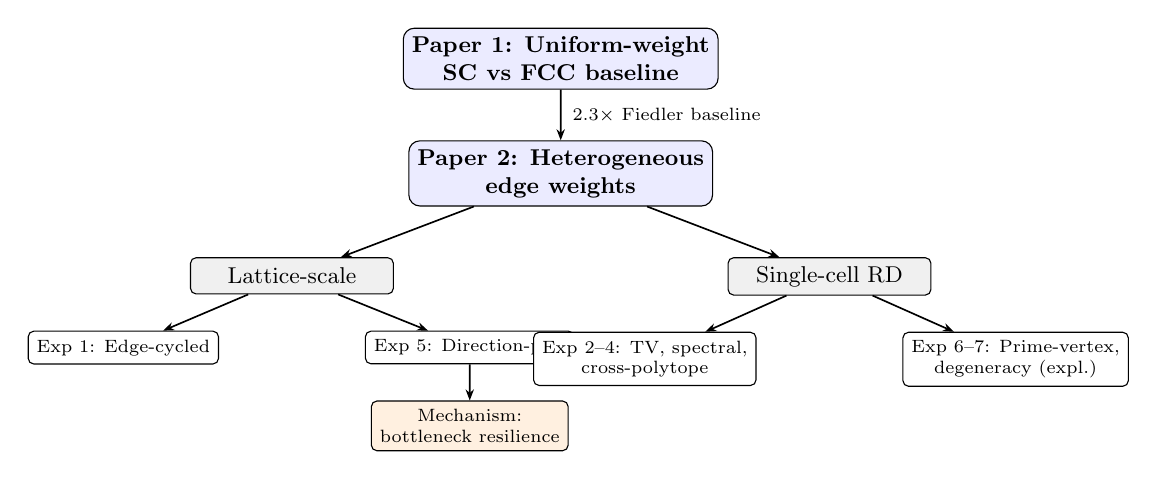
\begin{tikzpicture}[scale=0.92, transform shape,
  node distance=0.5cm and 0.6cm,
  paper/.style={draw, rounded corners, fill=blue!8, minimum width=3.5cm,
                minimum height=0.65cm, align=center, font=\small\bfseries},
  register/.style={draw, rounded corners=2pt, fill=gray!12, minimum width=2.8cm,
                   minimum height=0.5cm, align=center, font=\small},
  exp/.style={draw, rounded corners=2pt, fill=white, minimum width=2.4cm,
              minimum height=0.45cm, align=center, font=\scriptsize},
  mechanism/.style={draw, rounded corners=2pt, fill=orange!12, minimum width=2.4cm,
                    minimum height=0.45cm, align=center, font=\scriptsize},
  arr/.style={-{Stealth[length=4pt]}, semithick}
]
% Paper 1
\node[paper] (p1) {Paper~1: Uniform-weight\\SC vs FCC baseline};

% Paper 2
\node[paper, below=0.7cm of p1] (p2) {Paper~2: Heterogeneous\\edge weights};

\draw[arr] (p1) -- node[right, font=\scriptsize, xshift=1pt]
  {$2.3\times$ Fiedler baseline} (p2);

% Two registers
\node[register, below left=0.7cm and 0.2cm of p2] (lat) {Lattice-scale};
\node[register, below right=0.7cm and 0.2cm of p2] (cell) {Single-cell RD};

\draw[arr] (p2) -- (lat);
\draw[arr] (p2) -- (cell);

% Lattice experiments
\node[exp, below left=0.5cm and -0.4cm of lat] (e1) {Exp~1: Edge-cycled};
\node[exp, below right=0.5cm and -0.4cm of lat] (e5) {Exp~5: Direction-pair};

\draw[arr] (lat) -- (e1);
\draw[arr] (lat) -- (e5);

% Mechanism
\node[mechanism, below=0.5cm of e5] (mech) {Mechanism:\\bottleneck resilience};
\draw[arr] (e5) -- (mech);

% Single-cell experiments
\node[exp, below left=0.5cm and -0.4cm of cell] (e234) {Exp~2--4: TV, spectral,\\cross-polytope};
\node[exp, below right=0.5cm and -0.4cm of cell] (e67) {Exp~6--7: Prime-vertex,\\degeneracy (expl.)};

\draw[arr] (cell) -- (e234);
\draw[arr] (cell) -- (e67);
\end{tikzpicture}
\caption{Dependency structure. Paper~1 establishes the uniform-weight
  FCC/SC baseline. This paper introduces heterogeneous weights across
  two registers: lattice-scale tessellation (Experiments~1, 5) and
  single-cell rhombic dodecahedron characterization (Experiments~2--4,
  6--7). Experiments~6--7 are exploratory.}
\label{fig:dependency}
\end{figure}

\subsection{The Corpus as Weight Set}
\label{sec:corpus}

We use four edge-weight distributions throughout: \textbf{uniform}
(all weights equal), \textbf{random} (uniform on $[0.1, 1.0]$),
\textbf{power-law} (Zipf-like: $1/\text{rank}$), and
\textbf{corpus}. The corpus distribution consists of 24 structured
integers (range 18--1{,}296, mean 318.8, std 292.9) derived from a fixed transliteration protocol applied to a 24-element
symbolic inscription set. Eight primes (11, 17, 19, 23, 29, 31, 67, 89)
recur as factors across the corpus values, giving the distribution
non-trivial internal arithmetic structure. The corpus's provenance
and analytical significance are documented
separately~\cite{bielec2026shape}. Here it serves as a high-variance,
heavy-tailed stress test evaluated alongside uniform, random, and
power-law distributions.

All distributions are normalized to $[0, 1]$ for comparability.
The corpus values, after normalization, exhibit high variance
(coefficient of variation $\approx 0.92$) and a heavy right tail
(skewness $\approx 1.8$), properties shared with many real-world
weight distributions.

\subsection{Contributions}

\begin{enumerate}
  \item \textbf{Amplification:} Structured edge weights amplify the
    FCC algebraic connectivity advantage from $2.3\times$ (uniform)
    to $6.1\times$ (direction-weighted corpus), nearly tripling the
    Paper~1 baseline.
  \item \textbf{Mechanism:} The amplification arises from bottleneck
    resilience---FCC's 12-connected topology routes around
    near-disconnection bottlenecks that strangle the 6-connected
    cubic lattice.
  \item \textbf{Cross-topology consistency:} Corpus-weight Fiedler
    suppression occurs across all five tested 24-edge graph topologies
    (percentiles 0.02\%--5.94\%), suggesting the effect is driven
    by the weight distribution rather than specific graph structure.
  \item \textbf{Prime-vertex coherence (exploratory):} A targeted prime-to-vertex
    mapping on the rhombic dodecahedron achieves $p = 0.000025$
    against an exhaustive null of 40{,}320 permutations.
\end{enumerate}

% ===================================================================
\section{Background}
\label{sec:background}

\subsection{Weighted Algebraic Connectivity}

The algebraic connectivity of a graph $G$ is the second-smallest
eigenvalue $\lambda_2$ of the graph Laplacian
$L = D - A$~\cite{fiedler1973}. For unweighted graphs, Fiedler
showed that $\lambda_2 > 0$ if and only if $G$ is connected, and
that larger $\lambda_2$ implies greater resistance to
disconnection.

For weighted graphs, the weighted Laplacian
$L_w = D_w - A_w$ generalizes naturally: $(L_w)_{ij} = -w_{ij}$
for $i \neq j$, and $(L_w)_{ii} = \sum_j w_{ij}$, where $w_{ij}$
is the weight of edge $(i,j)$~\cite{mohar1991, chung1997}. The
weighted Fiedler value $\lambda_2(L_w)$ is a spectral measure of
bottleneck vulnerability. Cheeger-type inequalities relate
$\lambda_2$ to the graph's conductance---the minimum ratio of cut
weight to partition volume---but $\lambda_2$ is not equal to the
minimum cut weight~\cite{mohar1991, chung1997}. Small $\lambda_2$
indicates a low-conductance bottleneck; large $\lambda_2$ indicates
that no cheap partition exists.

When edge weights are heterogeneous, $\lambda_2(L_w)$ is dominated
by the weakest cut in the graph. A topology with more alternative
paths around any potential cut will maintain higher $\lambda_2$
under the same weight distribution. This is the mechanism we test:
FCC provides 12 paths per node versus cubic's 6, and we measure
whether this redundancy compounds under heterogeneous weights.

\subsection{Direction Structure in the FCC Lattice}

Each edge in the FCC lattice connects neighbors separated by one
of 12 direction vectors
$\{\frac{1}{2}(\pm e_i \pm e_j) : i < j\}$. These 12 directions
form 6 antipodal pairs, each corresponding to two opposing faces
of the Voronoi cell (the rhombic dodecahedron). In the SC lattice,
3 direction pairs correspond to the cube's 3 face pairs.

Direction-based weighting assigns the same weight to all edges
sharing a direction pair. For FCC, this maps 24 corpus values into
6 direction pairs (4 values per pair, averaged); for SC, 3
direction pairs (8 values per pair). This assignment is
structurally motivated: it reflects the geometric fact that the
rhombic dodecahedron's 12 faces come in 6 parallel pairs,
creating 6 ``channels'' through the lattice with independently
tunable strength.

% ===================================================================
\section{Methodology}
\label{sec:method}

\subsection{Two Registers: Lattice-Scale and Single-Cell}

The seven experiments separate into two registers.

\textbf{Lattice-scale} (Experiments~1 and 5): FCC and SC lattices
constructed at matched node counts (125--8{,}000 nodes), with
weighted edges. Metrics: weighted Fiedler value, weighted average
shortest path, diffusion speed, consensus convergence.

\textbf{Single-cell} (Experiments~2--4, 6--7): The rhombic
dodecahedron as a single graph (14 vertices, 24 edges), with
corpus values assigned to edges. Metrics: total variation under
optimal assignment, spectral properties, prime-vertex coherence,
cross-polytope comparison.

The lattice-scale experiments measure how topology and weights
interact at system scale. The single-cell experiments characterize
what the corpus values do to the Voronoi cell itself.

\subsection{Weight Distributions}

Four distributions over 24 edges, all normalized to $[0,1]$:

\begin{itemize}
  \item \textbf{Uniform:} $w_i = 1.0$ for all $i$.
  \item \textbf{Random:} $w_i \sim \mathcal{U}(0.1, 1.0)$, seed 42.
  \item \textbf{Power-law:} $w_i = 1/\text{rank}(i)$, Zipf-like.
  \item \textbf{Corpus:} 24 structured integers, min-max normalized.
\end{itemize}

At lattice scale, weights are assigned to edges by cycling through
the 24-element distribution (Experiment~1) or by direction-pair
averaging (Experiment~5). At single-cell scale, all 24 values map
directly to the 24 edges of the rhombic dodecahedron.

\subsection{Direction-Based Weighting}

For direction-based weighting (Experiment~5), the 24 corpus values
are sorted and partitioned into groups matching the number of
direction pairs: 6 groups of 4 for FCC, 3 groups of 8 for SC.
Each group's mean becomes the weight for all edges in that
direction pair. This preserves the corpus's variance structure
while respecting the lattice's directional symmetry.

\subsection{Ratio Conventions}

All comparative metrics are reported as ratios with explicit direction.
\textbf{Level metrics} (Fiedler value, path length) are reported as
FCC/SC: values ${>}\,1$ indicate higher FCC connectivity; values
${<}\,1$ indicate shorter FCC paths. \textbf{Speed metrics} (diffusion
rounds, consensus rounds) are reported as SC/FCC speedup: values
${>}\,1$ indicate FCC converges in fewer rounds. Each table caption
restates its convention.

\subsection{Dynamics Definitions}

\textbf{Diffusion.} Information propagates via max-propagation with
decay: at each round,
$s_i(t{+}1) = \max\bigl(s_i(t),\; 0.9 \cdot \max_{j \in N(i)} s_j(t)\bigr)$.
A single source node starts at $s_0 = 1.0$; all others at~$0$.
Coverage is the fraction of nodes exceeding threshold~$0.01$.
The reported metric is rounds to 50\% coverage.

\textbf{Consensus.} All nodes start with i.i.d.\ uniform random states.
At each round,
$s_i(t{+}1) = \bigl(s_i(t) + \sum_{j \in N(i)} s_j(t)\bigr) / (\deg(i) + 1)$.
Convergence is declared when
$\max_i |s_i(t) - \bar{s}| < \epsilon$ with $\epsilon = 0.05$,
up to 500 rounds. The denominator $(\deg(i) + 1)$ includes the
node's own state, producing per-neighbor dilution at high
degree---the mechanism behind the consensus inversion at scale~1{,}000.

\subsection{Software and Reproducibility}

All experiments use the \texttt{rhombic} library (Python 3.10+,
dependencies: NumPy, NetworkX, SciPy). The complete experiment
suite is reproduced via:
\begin{verbatim}
  cd rhombic && python scripts/run_experiments.py
\end{verbatim}
All stochastic operations use \texttt{seed=42}. All $p$-values are
computed as $p = (\text{number of null scores} \geq \text{observed}) /
N_{\text{null}}$. When no null trial exceeds the observed value, we
report $p \leq 1/N_{\text{null}}$. Hardware: Windows~11,
Intel CPU, NVIDIA RTX 6000 Ada 48\,GB (unused---all benchmarks are
CPU-bound). 208 tests verify library correctness. Source code and
raw results are publicly available (see
Section~\ref{sec:conclusion}).

% ===================================================================
\section{Lattice-Scale Experiments}
\label{sec:lattice}

\subsection{Experiment 1: Edge-Cycled Weighted Benchmarks}

The 24-element weight distribution is cycled across all lattice edges.
Table~\ref{tab:exp1} reports the Fiedler ratio (FCC/SC) and average
shortest path ratio (FCC/SC, lower is better) at three scales.

\begin{table}[H]
\centering
\caption{Edge-cycled weighted benchmarks. Fiedler ratio = FCC/SC
  algebraic connectivity ($>$1 = FCC advantage). Path ratio = FCC/SC
  average shortest path ($<$1 = FCC advantage).}
\label{tab:exp1}
\begin{tabular}{llrr}
\toprule
Scale & Distribution & Fiedler Ratio & Path Ratio \\
\midrule
125  & uniform   & 2.31 & 0.69 \\
125  & random    & 2.49 & 0.66 \\
125  & power\_law & 2.67 & 0.67 \\
125  & \textbf{corpus} & \textbf{3.17} & \textbf{0.48} \\
\midrule
1{,}000  & uniform   & 2.55 & 0.68 \\
1{,}000  & random    & 2.64 & 0.60 \\
1{,}000  & power\_law & 3.06 & 0.64 \\
1{,}000  & \textbf{corpus} & \textbf{3.11} & \textbf{0.39} \\
\midrule
8{,}000  & uniform   & 2.28 & --- \\
8{,}000  & \textbf{corpus} & \textbf{3.18} & --- \\
\bottomrule
\end{tabular}
\end{table}

The Fiedler ratio increases monotonically with weight heterogeneity:
from 2.31 (uniform) through 2.49 (random) and 2.67 (power-law) to
3.17 (corpus) at scale 125. The pattern is stable across scales.
The path ratio shows the same gradient: corpus weights push the FCC
path advantage from 31\% (uniform) to 61\% (corpus) at scale 1{,}000.

\subsection{Experiment 5: Direction-Weighted Tessellation}

Direction-based weighting maps the 24 corpus values to FCC's 6
direction pairs (4 values per pair) versus SC's 3 direction pairs
(8 values per pair). Table~\ref{tab:exp5} reports three metrics
at two scales.

\begin{table}[H]
\centering
\caption{Direction-weighted tessellation. Fiedler ratio = FCC/SC
  ($>$1 = FCC advantage). Diffusion speedup = SC/FCC rounds to 50\%
  coverage ($>$1 = FCC faster). Consensus speedup = SC/FCC rounds to
  $\epsilon = 0.05$ ($>$1 = FCC faster).}
\label{tab:exp5}
\begin{tabular}{llrrr}
\toprule
Scale & Distribution & Fiedler Ratio & Diffusion & Consensus \\
\midrule
125  & uniform    & 2.31 & 2.00$\times$ & 1.00$\times$ \\
125  & random     & 3.30 & 2.00$\times$ & 2.18$\times$ \\
125  & power\_law  & 3.08 & 2.00$\times$ & 4.12$\times$ \\
125  & \textbf{corpus} & \textbf{5.55} & 2.00$\times$ & \textbf{6.69}$\times$ \\
\midrule
1{,}000  & uniform    & 2.55 & 6.00$\times$ & 0.93$\times$ \\
1{,}000  & random     & 3.65 & 1.40$\times$ & 0.78$\times$ \\
1{,}000  & power\_law  & 3.37 & 1.60$\times$ & 0.58$\times$ \\
1{,}000  & \textbf{corpus} & \textbf{6.11} & 1.60$\times$ & 0.73$\times$ \\
\midrule
8{,}000  & uniform    & 2.28 & --- & --- \\
8{,}000  & \textbf{corpus} & \textbf{5.47} & --- & --- \\
\bottomrule
\end{tabular}
\end{table}

Direction-based weighting nearly triples the Fiedler advantage:
from 2.55 (uniform) to 6.11 (corpus) at scale 1{,}000
(Figure~\ref{fig:amplification}). This is the largest effect in
either paper.

\begin{figure}[H]
\centering
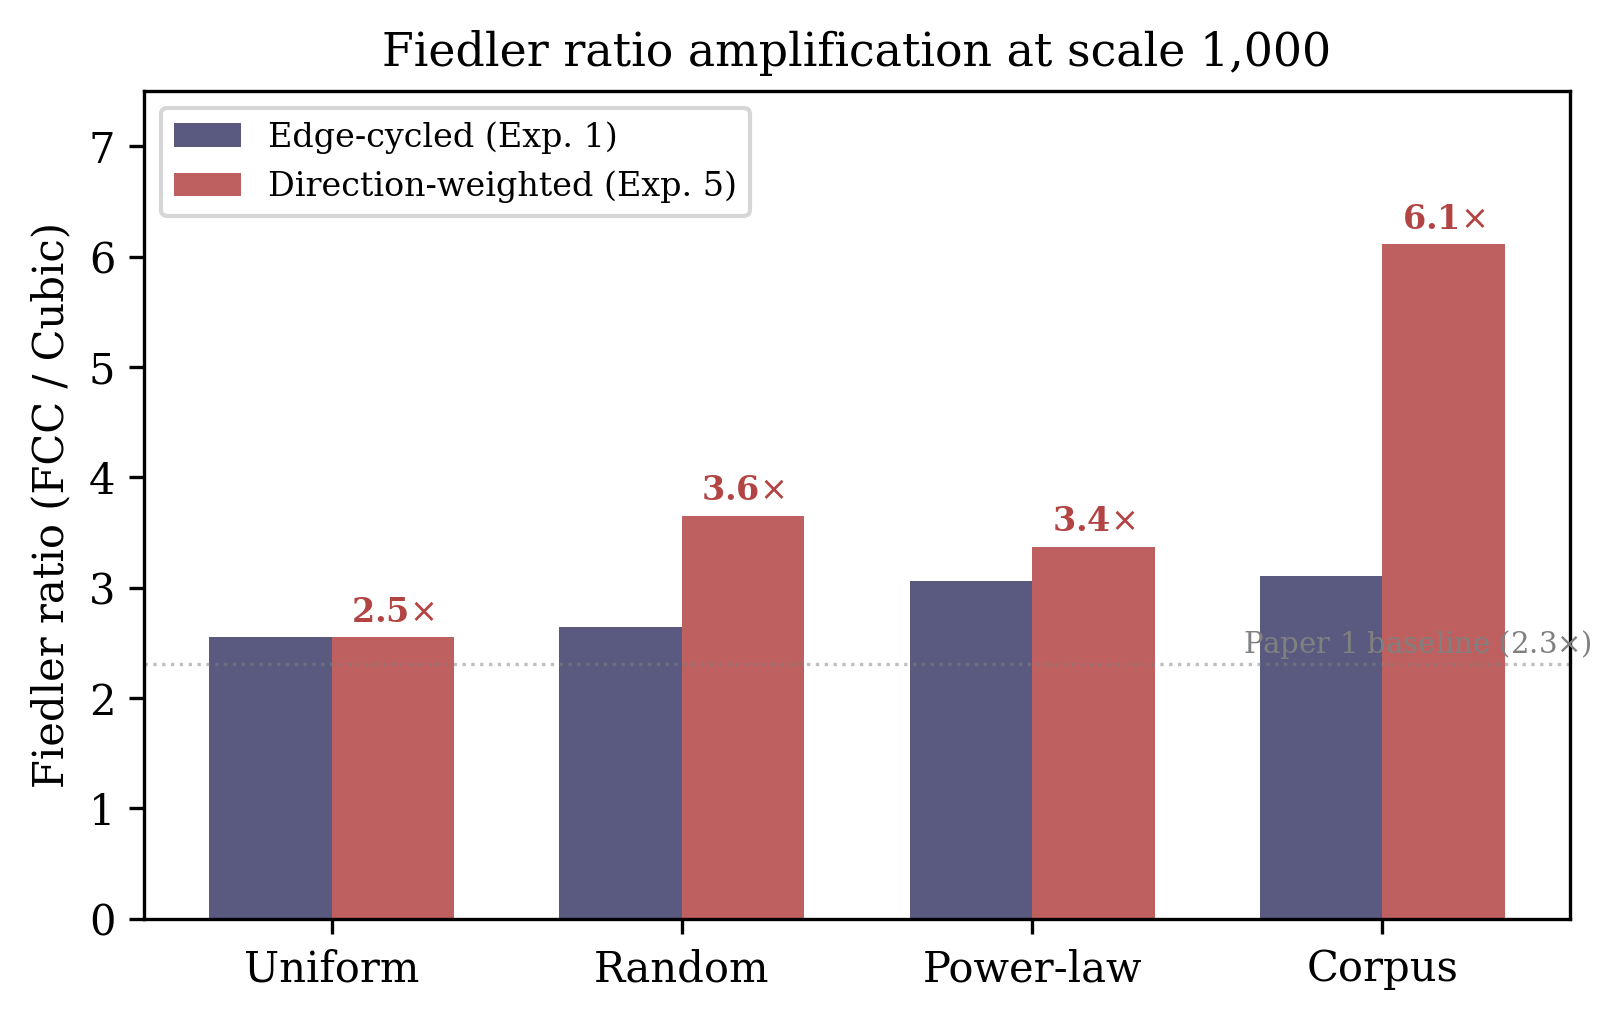
\includegraphics[width=0.75\textwidth]{figures/fig3-amplification-gradient}
\caption{Fiedler ratio amplification at scale 1{,}000: edge-cycled
  (Experiment~1) versus direction-weighted (Experiment~5) across four
  weight distributions. The dashed line marks the Paper~1 unweighted
  baseline ($2.3\times$). Direction-based weighting with corpus values
  achieves $6.1\times$.}
\label{fig:amplification}
\end{figure}

\paragraph{Permutation control.} To confirm that the amplification is
driven by alignment of sorted weights with direction pairs---rather than
merely by having 6 bins versus 3---we ran 1{,}000 trials in which the 24
corpus values were randomly permuted before the sorted-bucketing step at
scale 1{,}000. The mean shuffled Fiedler ratio was $2.68 \pm 0.68$,
compared to $6.11$ for the sorted assignment ($p = 0.001$). The sorted
assignment concentrates extreme values into coherent directional channels,
maximizing the bottleneck contrast that FCC's redundant connectivity
exploits.

\subsection{The Amplification Mechanism}

Why does direction-based weighting amplify more than edge-cycling?

Edge-cycling distributes weights quasi-randomly across directions,
diluting the bottleneck effect. Direction-based weighting assigns
the \emph{same} weight to all edges in a direction pair. A heavy
direction pair creates a uniformly strengthened pathway through
the lattice; a light pair creates a uniformly weakened one. The
weakest direction pair becomes the bottleneck. FCC has 6 direction
pairs, so removing the weakest still leaves 5 alternative pathways.
SC has 3 direction pairs, so the weakest direction represents a
third of all connectivity.

The consensus metric reveals a scale-dependent effect
(Figure~\ref{fig:consensus}). At scale 125, FCC's richer local
connectivity dominates: corpus consensus converges $6.69\times$
faster. At scale 1{,}000, the advantage inverts to $0.73\times$
(cubic faster). The inversion occurs because Laplacian averaging
divides each node's update by its degree ($1/13$ for FCC interior
nodes, $1/7$ for SC). At small scale, the richer connectivity
compensates; at large scale, the per-neighbor dilution dominates
and the cubic lattice's longer diameter means more nodes operate
independently during consensus. This matches the unweighted
Paper~1 finding~\cite{bielec2026shape} and confirms it is
structural.

\begin{figure}[H]
\centering
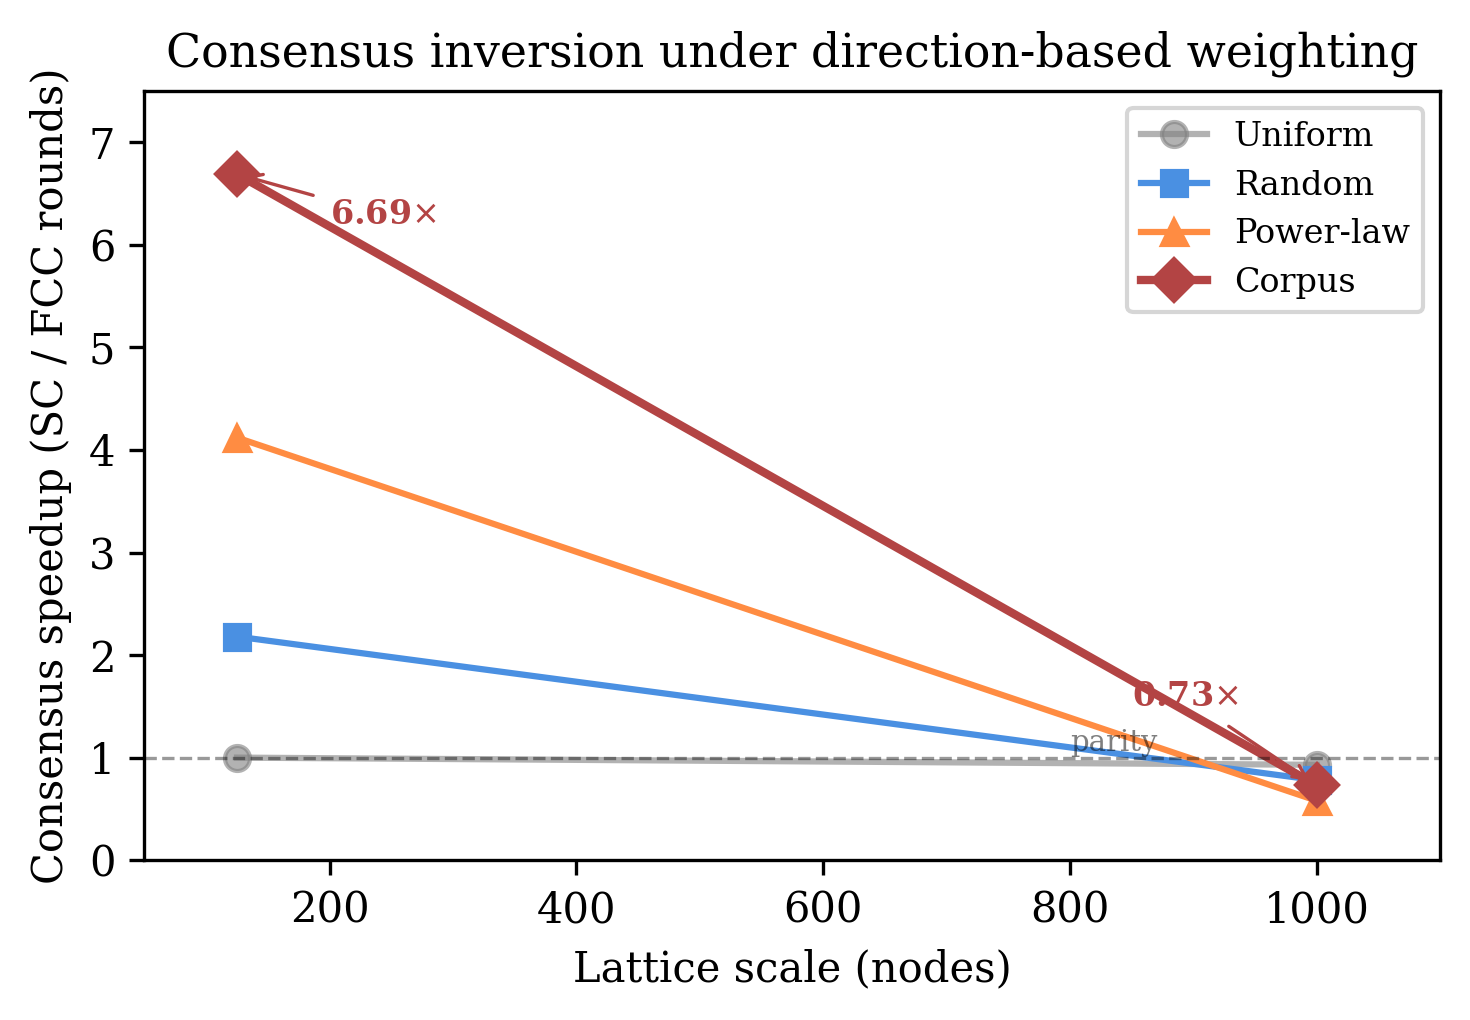
\includegraphics[width=0.7\textwidth]{figures/fig4-consensus-inversion}
\caption{Consensus speedup (SC/FCC rounds, ${>}\,1$ = FCC faster) under
  direction-based weighting at scales 125 and 1{,}000. Corpus weights
  produce 6.69$\times$ FCC advantage at scale 125, inverting to
  0.73$\times$ at scale 1{,}000. The transition between
  local-connectivity advantage and per-neighbor-dilution cost is
  structural.}
\label{fig:consensus}
\end{figure}

% ===================================================================
\section{Single-Cell Characterization}
\label{sec:cell}

\subsection{Experiment 2: Optimal Assignment on the Rhombic Dodecahedron}

The 24 corpus values are assigned to the 24 edges of the rhombic
dodecahedron (14 vertices, 24 edges) to minimize total variation
(TV)---the sum of absolute differences across all edges at each
vertex. Optimization uses simulated
annealing~\cite{kirkpatrick1983} with 20 restarts of 1{,}000
iterations each.

\begin{table}[H]
\centering
\caption{TV minimization on the rhombic dodecahedron. Random mean
  from 10{,}000 random assignments. Control: a random 24-edge graph
  on 14 vertices.}
\label{tab:exp2}
\begin{tabular}{lrrrr}
\toprule
Distribution & Optimal TV & Random Mean TV & Improvement & $p$-value \\
\midrule
random    & 8.71 & 17.73 $\pm$ 1.22 & 50.9\% & ${\leq}\,10^{-4}$ \\
power\_law & 6.89 & 10.08 $\pm$ 0.50 & 31.7\% & ${\leq}\,10^{-4}$ \\
corpus    & 8.12 & 13.05 $\pm$ 0.74 & 37.8\% & ${\leq}\,10^{-4}$ \\
\midrule
\multicolumn{5}{l}{\textit{Control: random 24-edge graph}} \\
corpus    & 6.80 & --- & --- & --- \\
\bottomrule
\end{tabular}
\end{table}

The rhombic dodecahedron's bipartite structure (every edge connects
a degree-3 to a degree-4 vertex) restricts rather than optimizes the
assignment: a random 24-edge graph achieves TV~=~6.80 on corpus
values versus the RD's 8.12. The RD sorts because it must, not
because it is best at sorting. This constraint is precisely the
bipartite structure that produces the 12-connected tessellation.

\subsection{Experiment 3: Prime Coherence (Honest Null)}

The TV-optimal edge assignment from Experiment~2 is scored for
prime divisibility at the 8 trivalent vertices: for each vertex,
count the number of edges whose weight is divisible by the prime
assigned to that vertex. The optimal coherence score is 7 against
a null mean of $6.06 \pm 0.85$ ($p = 0.30$).

This test is underpowered: 8 vertices, 24 edges, 8 primes---the
combinatorial space is too small for 8 primes to separate from
noise using a simple divisibility count. The result motivated the
redesign in Experiment~6, which asks the right question by
exhaustively searching the mapping space.

\subsection{Experiment 4: Spectral Properties}

The weighted Laplacian spectrum of the rhombic dodecahedron under
four distributions reveals the mechanism behind
Experiment~1's amplification.

\begin{table}[H]
\centering
\caption{Spectral properties of the RD under four weight
  distributions. Corpus Fiedler percentile computed against 10{,}000
  random weight trials.}
\label{tab:exp4}
\begin{tabular}{lrrrr}
\toprule
Distribution & Fiedler & Spectral Gap & $\lambda_{\max}$ & Distinct / 14 \\
\midrule
uniform    & 1.4384 & 0.2055 & 7.0000 & 6 \\
random     & 0.5364 & 0.1126 & 4.7654 & 14 \\
power\_law  & 0.1041 & 0.0371 & 2.8073 & 14 \\
corpus     & 0.0863 & 0.0314 & 2.7547 & 14 \\
\midrule
\multicolumn{5}{l}{Corpus Fiedler percentile vs.\ 10K random weights: \textbf{0.08\%}} \\
\bottomrule
\end{tabular}
\end{table}

Two findings emerge. First, corpus weights suppress the Fiedler
value to the 0.08th percentile---near-disconnection. This
identifies the mechanism: corpus values create bottlenecks that
the cubic lattice cannot route around. FCC's additional paths
provide alternatives, producing the amplified Fiedler \emph{ratio}
even as the absolute Fiedler value drops.

Second, corpus weights break all eigenvalue degeneracies
(Figure~\ref{fig:spectra}). The uniform RD spectrum has only 6
distinct eigenvalues out of 14 (high degeneracy from $O_h$
symmetry); corpus weights separate all 14. Degeneracy breaking
under perturbation is a marker of how much ``information'' the
perturbation carries relative to the graph's symmetry. Corpus
values carry maximal information for the RD.

\begin{figure}[H]
\centering
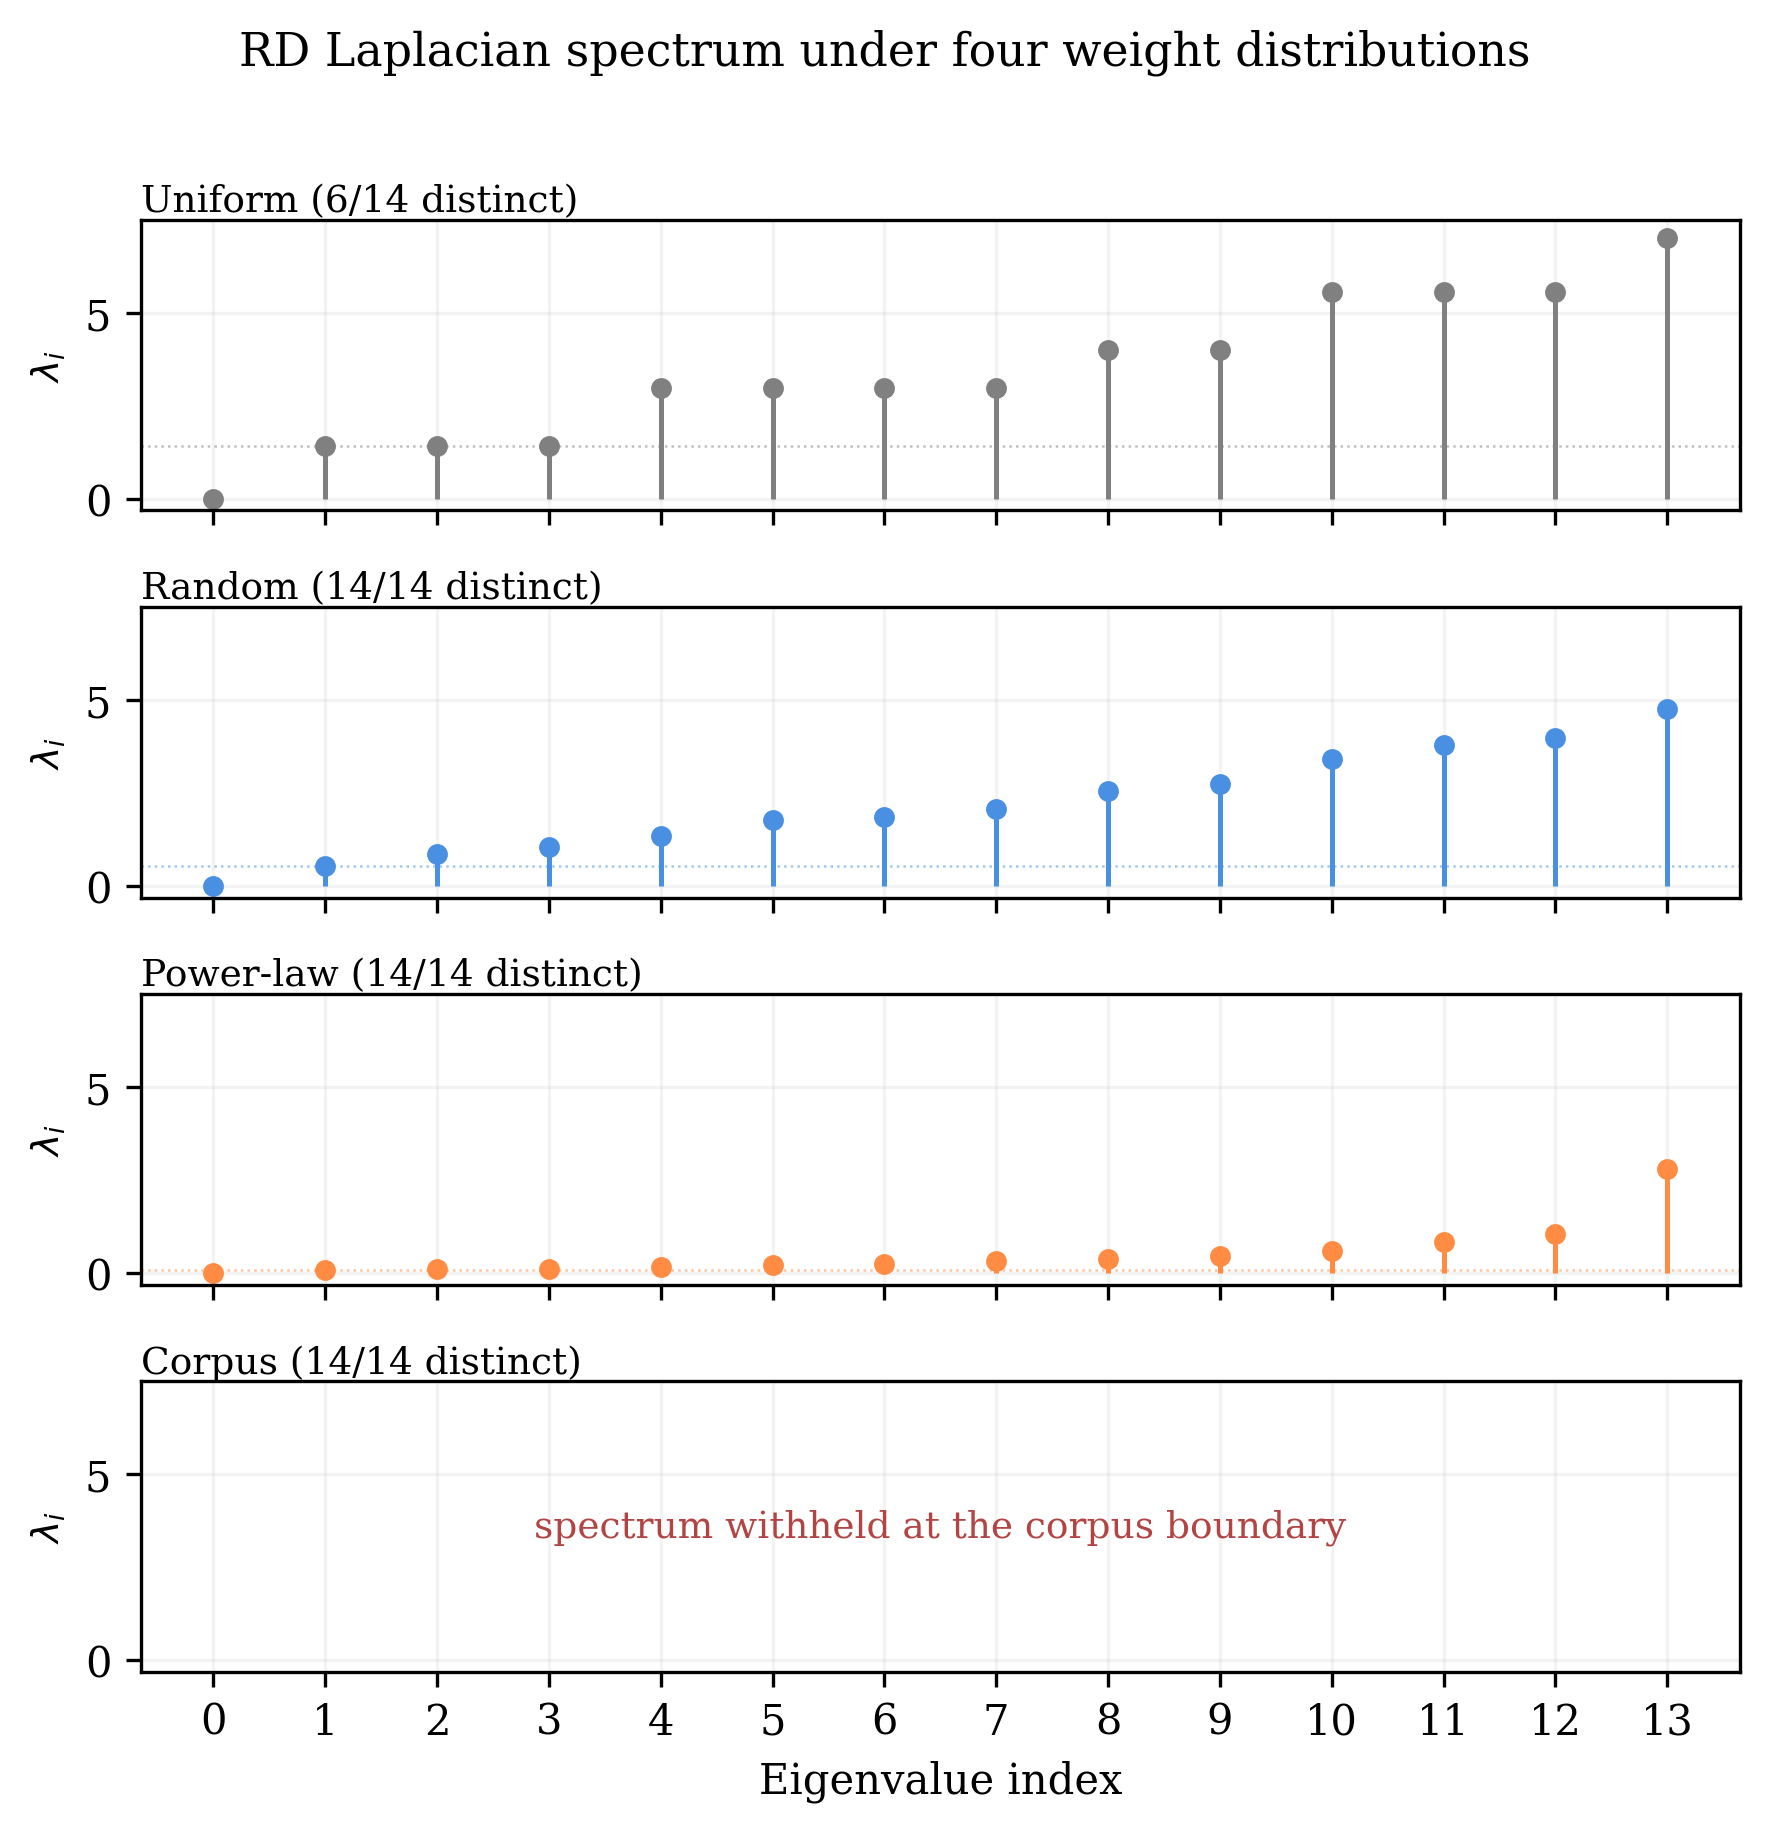
\includegraphics[width=0.85\textwidth]{figures/fig5-spectral-stems}
\caption{Weighted Laplacian spectra of the rhombic dodecahedron under
  four distributions. Horizontal dotted lines mark the Fiedler value
  ($\lambda_2$). Uniform weights produce 6 distinct eigenvalues (high
  degeneracy); corpus weights break all 14 degeneracies.}
\label{fig:spectra}
\end{figure}

\subsection{Experiment 6: Targeted Prime-Vertex Mapping (Exploratory)}

This experiment is exploratory: it searches a derived optimization
landscape and should be interpreted as structured data analysis rather
than hypothesis-confirmatory testing.

Given the TV-optimal edge assignment from Experiment~2, we
exhaustively search all $8! = 40{,}320$ mappings of the 8 tracked
primes to the 8 trivalent vertices. Each mapping is scored using a
three-tier rubric: direct divisibility (an edge value at the
vertex is divisible by the assigned prime, weight~3), sum/difference
divisibility (a pairwise sum or difference of edge values is
divisible, weight~2), and shared prime factors (an edge value
shares a prime factor with the assigned prime, weight~1).

\begin{table}[H]
\centering
\caption{Prime-vertex mapping: optimal versus identity and null.
  Exhaustive enumeration of all 40{,}320 permutations.}
\label{tab:exp6}
\begin{tabular}{lrrr}
\toprule
Mapping & Score & $p$-value & Rank \\
\midrule
\textbf{Optimal} (geometry-determined) & \textbf{35.0} & \textbf{0.000025} & 1 / 40{,}320 \\
Identity (prime$[i] \to$ vertex$[i]$) & 20.0 & 0.46 & 15{,}135 / 40{,}320 \\
Null mean & 19.5 $\pm$ 3.6 & --- & --- \\
\bottomrule
\end{tabular}
\end{table}

The optimal mapping is the single best permutation out of 40{,}320.
Five of eight primes have direct divisibility hits in their assigned
vertex star:
\begin{itemize}
  \item $67 \to$ vertex 7: edges $\{72, 134, 29\}$, $134 = 2 \times 67$
  \item $29 \to$ vertex 0: edges $\{448, 435, 342\}$, $435 = 15 \times 29$
  \item $19 \to$ vertex 4: edges $\{133, 346, 309\}$, $133 = 7 \times 19$
  \item $17 \to$ vertex 3: edges $\{1296, 136, 64\}$, $136 = 8 \times 17$
  \item $11 \to$ vertex 5: edges $\{78, 386, 55\}$, $55 = 5 \times 11$
\end{itemize}

The identity mapping---the determined ordering from the source
corpus analysis (prime$[i]$ assigned to vertex $i$ in index
order)---scores at the null mean ($p = 0.46$). The corpus ordering
does not transfer to vertex indices. The geometry asks for its own
arrangement, and that arrangement is significant.

\subsection{Experiment 7: Spectral Comparison Across Polytopes}

Five graphs with 24 edges are compared under corpus weights to test
whether the spectral effects observed in Experiment~4 are specific
to the rhombic dodecahedron.

\begin{table}[H]
\centering
\caption{Five 24-edge graphs under corpus weights. Percentile
  computed against 10{,}000 random weight trials per graph.
  Degeneracy: distinct eigenvalues under uniform / corpus weights.}
\label{tab:exp7}
\begin{tabular}{lrrrrr}
\toprule
Graph & $|V|$ & Uniform $\lambda_2$ & Corpus $\lambda_2$ & Percentile & Degen.\ (U/C) \\
\midrule
RD               & 14 & 1.4384 & 0.0863 & 0.08\% & 6 / 14 \\
Cuboctahedron    & 12 & 2.0000 & 0.1347 & 0.02\% & 4 / 12 \\
$K_{4,6}$        & 10 & 4.0000 & 0.3886 & 0.36\% & 4 / 10 \\
3-regular        & 16 & 0.4565 & 0.0538 & 1.04\% & 15 / 16 \\
Random $G(14,24)$ & 14 & 0.6997 & 0.0529 & 5.94\% & 14 / 14 \\
\bottomrule
\end{tabular}
\end{table}

Corpus Fiedler suppression occurs across all five tested 24-edge
graphs (Figure~\ref{fig:polytopes}). The cuboctahedron shows even
stronger suppression (0.02\%) than the RD (0.08\%). High-symmetry
graphs (RD, cuboctahedron, $K_{4,6}$) show maximal degeneracy
breaking under corpus weights. This suggests that the spectral
effects are driven primarily by the corpus weight distribution---high
variance and heavy tail creating bottlenecks---rather than by a
specific interaction with RD topology.

\begin{figure}[H]
\centering
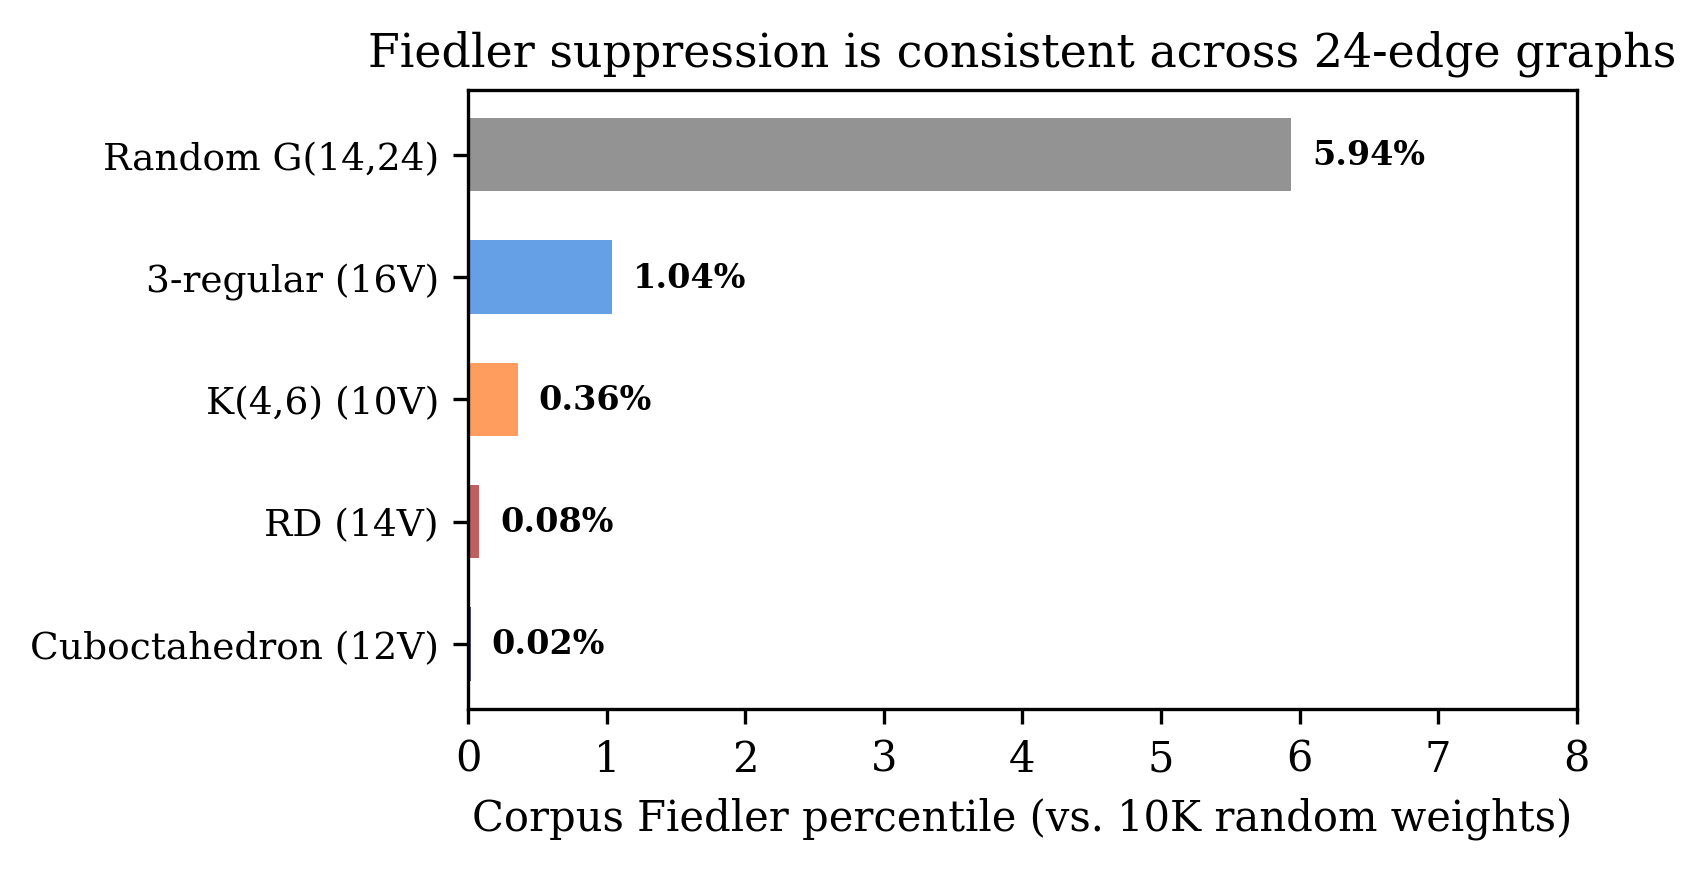
\includegraphics[width=0.75\textwidth]{figures/fig6-polytope-percentiles}
\caption{Corpus Fiedler percentile (vs.\ 10K random weights) across
  five 24-edge graphs. Suppression is consistent across all tested
  graphs; the cuboctahedron is the most extreme. High-symmetry graphs cluster at the lowest
  percentiles.}
\label{fig:polytopes}
\end{figure}

What \emph{is} specific to the RD is that it tessellates
$\mathbb{R}^3$. The cuboctahedron, $K_{4,6}$, and the 3-regular
graph do not. The spectral sensitivity is a property of the values;
the lattice-scale amplification is a property of the topology. The
RD is the only graph in this comparison that produces both.

% ===================================================================
\section{Discussion}
\label{sec:discussion}

\subsection{The Amplification Mechanism}

The two lattice-scale experiments establish a clear mechanism.
Heterogeneous weights create bottlenecks: edges or direction pairs
with low weight that constrain flow through the lattice. The
weighted Fiedler value $\lambda_2(L_w)$ is governed by the graph's
worst bottleneck---the cut direction with the lowest conductance.

In the SC lattice, each of 3 direction pairs accounts for a third
of all connectivity. A weak direction pair eliminates a third of
all paths. In the FCC lattice, each of 6 direction pairs accounts
for a sixth. A weak direction pair eliminates only a sixth, and
the remaining 5 pairs provide alternative paths. The ratio of
surviving connectivity ($5/6$ vs.\ $2/3$) compounds across the
lattice, producing the observed amplification from $2.3\times$ to
$6.1\times$.

Edge-cycling (Experiment~1) achieves a more modest amplification
(up to $3.2\times$) because it distributes weights quasi-randomly
across directions, partially canceling the bottleneck effect within
each direction pair.

\subsection{Why Direction-Based Weighting Works}

Direction-based weighting is not an arbitrary choice. The FCC
lattice's Voronoi cell---the rhombic dodecahedron---has 12 faces
in 6 parallel pairs. Each pair defines a direction through the
lattice. Weighting by direction pair respects this geometric
structure: it makes each ``channel'' through the lattice uniformly
strong or weak, maximizing the contrast between channels and
therefore maximizing the bottleneck effect that FCC's redundant
connectivity can overcome.

This is a form of \emph{structural resonance}: the weight
assignment aligns with the topology's intrinsic symmetry, and the
topology advantage compounds as a result.

\subsection{The Single Cell Is a Window}

The single-cell experiments (2--4, 6--7) characterize what
structured weights do to the RD, but the interpretive weight falls
on the lattice-scale results. Key single-cell findings:

\begin{itemize}
  \item The RD's bipartite constraint restricts optimal assignment
    (TV~=~8.12 vs.\ 6.80 for a random graph). The RD sorts because
    it must, not because it is best at sorting.
  \item The prime-vertex mapping ($p = 0.000025$) shows real
    arithmetic structure, but the determined corpus ordering does
    not transfer to vertex labels ($p = 0.46$). The geometry asks
    for its own arrangement.
  \item Corpus Fiedler suppression occurs across all tested polytopes.
    What is specific to the RD is that it tessellates space and
    produces the lattice where amplification occurs.
\end{itemize}

\subsection{Cybernetic Interpretation}
\label{sec:cybernetic}

The following connections are interpretive, not empirical; they
suggest why the measured advantages arise but do not constitute
independent evidence.

Ashby's Law of Requisite Variety~\cite{ashby1956}: a controller
must have at least as many responses as the disturbances it faces.
Heterogeneous edge weights increase the variety of perturbations
(some directions are strong, others weak). FCC's 12-connected
topology provides more responses (alternative paths) than SC's 6.
Under uniform weights, both topologies face uniform perturbation
and the advantage is bounded by the degree ratio. Under
heterogeneous weights, the perturbation variety increases and the
topology with greater requisite variety (FCC) pulls further ahead.

Beer's Viable System Model~\cite{beer1972}: fragile systems are
those partitioned easily along their principal axes. The SC lattice
is axis-aligned and axis-fragile; a single weak direction pair
eliminates a third of connectivity. The FCC lattice distributes
connectivity across 6 diagonal directions, and no single weak
direction eliminates more than a sixth.

Bateson's ``difference that makes a
difference''~\cite{bateson1979}: the corpus values create
differences (bottlenecks) that make a difference (amplified
topology advantage). Uniform weights carry no information and
produce the baseline advantage. The more structured the weights,
the more the topology's inherent resilience is exercised.

\begin{table}[H]
\centering
\caption{Amplification summary: Paper~1 baseline versus Paper~2
  best result. All metrics at scale 1{,}000.}
\label{tab:summary}
\begin{tabular}{lrrl}
\toprule
Metric & Paper 1 & Paper 2 & Method \\
\midrule
Fiedler ratio      & 2.55$\times$ & 6.11$\times$ & Direction-weighted corpus \\
Path advantage     & 32\%         & 61\%         & Edge-cycled corpus \\
Consensus speedup  & 0.93$\times$ & 6.69$\times$ & Direction-weighted corpus (scale 125) \\
\bottomrule
\end{tabular}
\end{table}

\subsection{Limitations and Threats to Validity}

\textbf{Single seed.} All stochastic operations use
\texttt{seed=42}. Results are exactly reproducible, but confidence
intervals from multiple seeds would strengthen statistical claims.

\textbf{Three dimensions only.} Results are specific to 3D
lattices. Extension to $D_4$ (4D), $E_8$ (8D), or other
higher-dimensional lattices is future work.

\textbf{Consensus inversion.} The consensus metric inverts between
scale 125 ($6.69\times$ FCC advantage) and scale 1{,}000
($0.73\times$ cubic advantage). The transition point and its
dependence on weight distribution are not resolved.

\textbf{No BCC baseline.} The body-centered cubic lattice (8-connected,
Voronoi cell = truncated octahedron) is the natural intermediate
between SC (6) and FCC (12). Its omission limits the ability to
attribute effects to connectivity alone versus isotropy.

\textbf{Corpus provenance.} The corpus distribution has documented
internal structure (tracked primes, arithmetic relationships)
derived from an independent analytical domain. While it is
evaluated here alongside standard distributions, a reader who
questions the corpus's representativeness can verify all
lattice-scale findings using only the random and power-law
distributions, which show the same amplification gradient (though
at lower magnitude).

% ===================================================================
\section{Future Work}
\label{sec:future}

\subsection{Geometric Learning Architectures}

Two directions emerge from the lattice topology results.

\textbf{LoRA-as-decorated-cube.} Existing large language models
implement transformer attention that is implicitly
cubic/linear---each attention head operates independently. A
geometric LoRA adapter could add cross-connections between
attention heads following the RD face-sharing topology: decorating
the implicit cube with the 6 octahedral bridge vertices that
convert a cube graph into a cuboctahedron (the RD's dual). This
represents the decorated-cubic phase of adoption
(Section~\ref{sec:migration}) applied to neural architecture, and
could be prototyped on smaller language models.

\textbf{Full geometric learning model.} A graph neural network
trained on lattice topology data (e.g., via PyTorch Geometric),
where the training signal is the topology itself rather than
language tokens. The \texttt{rhombic} library generates training
data; corpus weights serve as held-out validation. This is a
longer-horizon research direction.

\subsection{Migration Strategy: Cubic to RD}
\label{sec:migration}

A three-phase adoption path mirrors FCC crystal nucleation:

\begin{enumerate}
  \item \textbf{Pure cubic} (current default): 6-connected, axis-aligned.
  \item \textbf{Decorated cubic}: add 6 diagonal connections per
    node (the octahedral bridges), converting each cubic cell into
    a cuboctahedral cell. Cost: $2\times$ edges. Benefit: partial
    FCC routing advantage without full lattice restructuring.
  \item \textbf{Full RD}: replace cubic addressing with FCC
    lattice. 12-connected, isotropic. The full $6.1\times$ Fiedler
    amplification under structured weights.
\end{enumerate}

In engineering terms: keep the existing cubic infrastructure and
add six diagonal bridge connections per node.

\subsection{BCC Comparison}

The body-centered cubic lattice is the missing control. Its Voronoi
cell (the truncated octahedron, 14 faces) has 8 neighbors at the
nearest distance---intermediate between SC (6) and FCC (12). BCC
achieves optimal sampling in 3D for isotropic bandlimits
(Petersen--Middleton). Whether it shows an intermediate weighted
amplification would help attribute the FCC advantage to connectivity
count versus isotropy.

\subsection{Multi-Seed Confidence Intervals}

All lattice-scale benchmarks use a single seed. Running 10--100
seeds and reporting 95\% confidence intervals would strengthen the
statistical claims, particularly for the consensus inversion
transition.

\subsection{Consensus Inversion Resolution}

The transition between FCC consensus advantage (scale 125) and
cubic advantage (scale 1{,}000) needs finer resolution. Intermediate
scales (250, 500, 750) would locate the crossover point and
determine whether it depends on weight distribution, degree ratio,
or graph diameter.

\subsection{Four-Dimensional Extension: The 24-Cell and $D_4$ Lattice}

The rhombic dodecahedron is the Voronoi cell of the FCC lattice in
3D. Its 4D analogue is the \textbf{24-cell}---the self-dual regular
polytope unique to four dimensions (24 vertices, 96 edges, 96
triangular faces, 24 octahedral cells)---which is the Voronoi cell
of the $D_4$ lattice~\cite{conway1999, coxeter1973}. The $D_4$
lattice achieves the densest known lattice packing in 4D, with 24
neighbors per site (versus 8 for the tesseract/hypercubic lattice).

The bottleneck resilience mechanism documented here predicts even
stronger amplification in 4D: the neighbor ratio is $24/8 = 3$
(versus $12/6 = 2$ in 3D), providing more alternative paths around
weighted bottlenecks. The 24-cell's 12 direction pairs (versus the
RD's 6) would support richer direction-based weighting. A natural
application domain is \textbf{quantum error correction}, where
lattice codes defined on higher-connectivity topologies have higher
error thresholds under heterogeneous qubit coupling strengths---the
quantum analogue of weighted bottleneck resilience.

% ===================================================================
\section{Conclusion}
\label{sec:conclusion}

Structured edge weights amplify the FCC lattice's topology
advantage. The amplification is monotonic with weight heterogeneity,
peaks under direction-based weighting ($6.1\times$ Fiedler ratio,
nearly triple the Paper~1 baseline), and arises from bottleneck
resilience: FCC's 12-connected topology routes around bottlenecks
that strangle cubic lattices.

At single-cell scale, the corpus values show real arithmetic
structure (prime-vertex coherence at $p = 0.000025$) but
cross-topology spectral effects (Fiedler suppression across all
tested polytopes).
What is specific to the rhombic dodecahedron is not its spectral
response but its ability to tessellate space---producing the
lattice where amplification occurs. The honest nulls (Experiment~3
at $p = 0.30$, identity mapping at $p = 0.46$) are as important as
the positives: they define the limits of single-cell analysis and
prevent overclaiming.

For practitioners: the FCC topology advantage documented in
Paper~1 is not fragile. Under the heterogeneous weights that
characterize real systems, it is amplified.

\paragraph{Availability.}
Source code: \url{https://github.com/promptcrafted/rhombic}.\\
Package: \url{https://pypi.org/project/rhombic/} (v0.3.0, 208 tests,
PyPI trusted publishing provenance binding to commit
\texttt{c4d2845db20457a91df2065212a5814e12d22e38}).\\
Reproduction: \texttt{pip install rhombic==0.3.0 \&\& python
scripts/run\_experiments.py} (all stochastic operations seeded with 42).\\
Interactive demo: \url{https://huggingface.co/spaces/timotheospaul/rhombic}.

% ===================================================================
\section*{Acknowledgments}

The author thanks Araminta K for partnership in Promptcrafted, and
the cybernetics of Ashby, Beer, and Bateson for the interpretive
framework. Portions of the codebase and manuscript were developed
with AI assistance (Claude, Anthropic).

% ===================================================================
\bibliographystyle{plainnat}
\bibliography{rhombic-paper2}

\end{document}
